\chapter{Model-View-Controller}

\section{Summary}
Das Model-View-Control-Pattern (MVC) teilt eine Applikation in drei Komponenten, wobei Programmlogik und Daten von der Präsentation getrennt werden. Ein Change-Progragation-Mechanismus sorgt dafür, dass die Daten zwischen den Schichten konsistent bleiben.
\section{Context}
Interaktive Applikationen mit einem flexiblen User-Interface.
\section{Problem}
User-Interfaces (UI) verursachen viel Arbeit. Wenn neue Features entwickelt werden, müssen dazu UIs entwickelt werden, ein Kunde möchte eine spezifische Änderung der Benutzerführung oder die Applikation muss auf eine andere Plattform mit einem anderen \textit{look and feel} portiert werden. 

Einem System die benötigte Flexibiltät zu geben, kann teuer und fehleranfällig werden, wenn das UI eng mit der Programmlogik verknüpft ist. Es kann dazu führen, dass verschiedene Softwaresysteme parallel gepflegt werden müssen, eines für jede UI-Implementation.

Folgende Forces beeinflussen die Lösungen zu solchen Problemen:
\begin{itemize}
	\item Die gleichen Informationen müssen auf verschiedene Weise präsentiert werden (z.B. Balken- oder Kuchendiagramm)
	\item Die Darstellung oder das verhalten einer Applikation müssen sofort auf veränderte Daten reagieren
	\item Änderungen am UI sollten einfach und sogar zur Laufzeit möglich sein
	\item Verschiedene \textit{look and feel} Standards oder eine Portierung des UIs sollten den Code der Kernfunktionalität der Applikation nicht beeinflussen
\end{itemize}

\section{Solution}
MVC teilt die Applikation in drei Bereiche: \textit{Verarbeitung}, \textit{Output} und \textit{Input}. 

Die \textbf{Model}-Komponente kapselt die Daten und Kernfunktionalität. Das Model ist unabhängig von spezifischen Datenrepräsentationen oder Eingabeverhalten

\textit{View}-Komponenten zeigen die Informationen dem Benutzer an. Eine View erhält die Daten vom Model. Zu einem Model können mehrere Views existieren

Jede View hat eine dazugehörige \textit{Controller}-Komponente. Controller wandeln den Input des Benutzers (Mausbewegungen, Mausklicks, Tastatureingaben) in Service Requests für das Model oder die View um. Der Benutzer interagiert mit dem System nur über Controller.

Diese Trennung ermöglicht es, für ein Model mehrere Views zu haben. Wenn nun der Benutzer über den Controller Daten im Model ändert, müssen alle anderen Views dieses Models diese Änderungen auch anzeigen. Deshalb benachrichtigt das Model alle Views über Änderungen. Dies wird durch das Publisher-Subscriber-Pattern gelöst.

Die nachfolgende Grafik zeigt den Zusammenhang zwischen Model, View und Controller:

\begin{figure}[H]
	\centering
	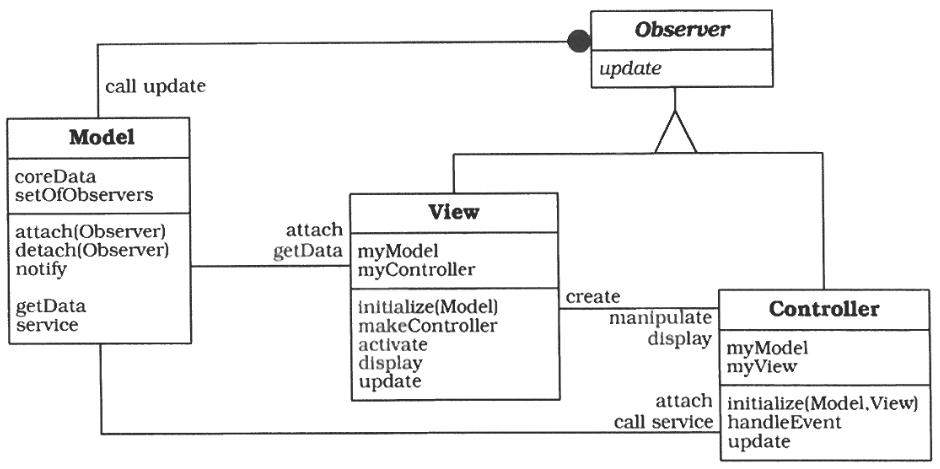
\includegraphics[width=0.8\textwidth]{figures/03-mvc-1}
	\caption{Zusammenhang zwischen MVC-Komponenten}
\end{figure}


\section{Consequences}
\begin{itemize}
    \pro{Mehrere Views für ein Model}
    \pro{Synchronisierte Views}
    \pro{Auswechselbare Views und Controller, sogar zur Laufzeit}
    \pro{Austauschbarkeit des \textit{look and feel}}
    \pro{Auf diesem Pattern kann ein Framework aufgebaut werden}
    \con{Erhöhte Komplexität}
    \con{Eine einzelne Aktion des Benutzers kann eine übermässige Anzahl Updates auslösen}
    \con{Controller und View sind sehr eng verzahnt, was deren einzelne Wiederverwertbarkeit erschwert}
    \con{Views und Controller sind stark an ein Model gekoppelt $\rightarrow$ Änderungen am Model erfordern Änderung an Views und Controller}
    \con{Ineffiziente Datendarstellung: Je nach Interface des Models müssen mehrere Requests gemacht werden, um das Interface aufzubauen}
\end{itemize}

\section{Known Uses}
\begin{itemize}
	\item \textbf{Smalltalk:} Das User Interface Framework in Smaltalk
	\item \textbf{MFC:} Die Document-View-Variation von MVC dient in C++ als Basis für Windows-Applikationen
	\item \textbf{ET++:} Das Applikations-Framework ET++ arbeitet auch mit einer Document-View-Variation
\end{itemize}

\section{Relationships}
\begin{itemize}
	\item Das \textit{Presentation-Abstraction-Control}-Pattern zeigt einen anderen Ansatz um das User Interface vom funktionalen Kern einer Applikation zu trennen.
\end{itemize}

\section{Exam Questions}
\begin{itemize}
  \item Behauptung: dies ist eine Behauptung? (Lösung)
    \item Frage: Dies ist eine Frage? (Lösung)
\end{itemize}
